% =================================================
% Chapter 5 — Wet Well Recommendations
% =================================================

\section{Wet Well Recommendations}

% -------------------------------------------------
\subsection{Introduction to Wet Well Design}
% -------------------------------------------------

Once the system curve has been established and the selected pump has been matched to that system, the next step is to size the wet well and define the operating control elevations. For the Colebrooke Subdivision lift station, the selected pump is the Sulzer XFP100C VX 1$\sim$ (wet pit) with vortex impeller. The selected operating point from the pump selection process is $135.5~\text{gpm}$ at $12.08~\text{ft}$ of head, and the system inflow to the wet well at peak conditions is $12.46~\text{gpm}$. These values were used to size the minimum storage volume and define the control elevations for the duplex wet well. The project itself includes pump station design and force main design as one of the major infrastructure components of the subdivision \cite{ProjectD_Colebrooke_2020}, and the working inflow and pump discharge values used in the wet well sketches are shown in the reference figures prepared for this design.

The conceptual arrangement of the wet well and pump configuration is illustrated in Figure~\ref{fig:wetwell_storage_config}.

\begin{figure}[H]
\centering
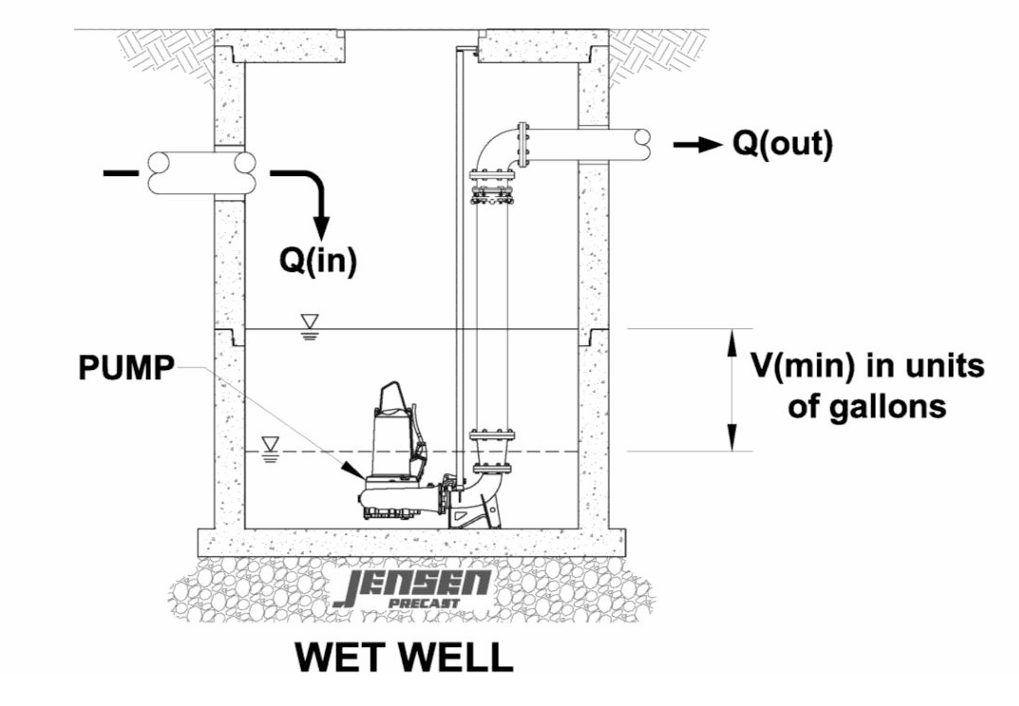
\includegraphics[
width=0.85\textwidth
]{calc_vmin.png}
\caption{Wet well storage and pumping configuration showing inflow, pump intake, and storage volume concept.\cite{Jensen_PumpStationDesignGuidelines_2012}}
\label{fig:wetwell_storage_config}
\end{figure}

As shown in Figure~\ref{fig:wetwell_storage_config}, the wet well receives an inflow of $12.46~\text{gpm}$ and the selected pump discharges at $135.50~\text{gpm}$, which creates the active storage and drawdown region used in the minimum storage calculation.

The design inflow rate to the wet well was determined from the projected wastewater flow for the subdivision, while the discharge rate corresponds to the operating point determined from the pump selection process. The resulting wet well configuration ensures reliable wastewater conveyance to the downstream gravity sewer system located at elevation $309.28~\text{ft}$, as illustrated in the system profile drawing \cite{ProjectD_Colebrooke_2020}.

% -------------------------------------------------
\subsection{Minimum Storage Volume}
% -------------------------------------------------

Wet well storage volume is designed to ensure that pumps do not start and stop excessively. Frequent pump cycling can cause increased mechanical wear, higher electrical loads, and reduced pump life. For low-flow lift stations, Jensen recommends sizing the wet well so that the time between pump starts is approximately $8$--$10$ minutes, while also verifying that the selected pump does not exceed the allowable number of starts per hour \cite{Jensen_PumpStationDesignGuidelines_2012}. The Sulzer pump data indicate a maximum of $15$ starts per hour, which corresponds to an absolute minimum interval of about $4$ minutes between starts. The selected design therefore satisfies the manufacturer limit if the cycle time is kept at $10$ minutes.

The minimum storage volume was calculated using the general Hydraulic Institute cycle-time relationship rather than the Jensen simplification $Q_{in}=Q_{out}/2$, because the actual inflow and selected pump discharge are already known for this project. Using the notation of the guideline, the cycle time is

\[
\begin{aligned}
T_{min} &= \frac{V_{min}}{Q_{in}} + \frac{V_{min}}{Q_{out}-Q_{in}}
\end{aligned}
\]

where $Q_{in}=12.46~\text{gpm}$, $Q_{out}=135.50~\text{gpm}$, and $T_{min}=10~\text{min}$.

First, the net pumping rate during pump operation is

\[
\begin{aligned}
Q_{out}-Q_{in} &= 135.50-12.46 \\
&= 123.04~\text{gpm}
\end{aligned}
\]

Substituting into the cycle-time equation gives

\[
\begin{aligned}
10 &= \frac{V_{min}}{12.46}+\frac{V_{min}}{123.04} \\
10 &= V_{min}\left(\frac{1}{12.46}+\frac{1}{123.04}\right) \\
10 &= V_{min}(0.08026+0.00813) \\
10 &= V_{min}(0.08839) \\
V_{min} &= \frac{10}{0.08839}=113.1~\text{gal}
\end{aligned}
\]

Thus, the minimum storage volume required to maintain a $10$-minute cycle time is

\[
\boxed{V_{min}=113~\text{gal}}
\]

This value, however, only satisfies the cycle-time requirement. A run-time check was then performed because a very small wet well volume can cause the pump to start and stop too quickly. The pump-on run time corresponding to $V_{min}=113~\text{gal}$ is

\[
\begin{aligned}
t_{on} &= \frac{V}{Q_{out}-Q_{in}} \\
&= \frac{113.1}{123.04}=0.919~\text{min}
\end{aligned}
\]

\[
\begin{aligned}
t_{on} &= 0.919\times 60 \\
&= 55.1~\text{s}
\end{aligned}
\]

A run time of $55.1~\text{s}$ is short for a submersible wastewater pump, even though the starts-per-hour criterion is technically met. In the absence of a stricter minimum run-time value from the manufacturer, a $2$-minute minimum run time was adopted as a conservative engineering design value for wet well sizing. Using this criterion, the required active storage becomes

\[
\begin{aligned}
V &= (Q_{out}-Q_{in})t_{on} \\
&= 123.04\times 2 \\
&= 246.08~\text{gal}
\end{aligned}
\]

For design purposes, this was rounded to

\[
\boxed{V_{min,\ design}=250~\text{gal}}
\]

Accordingly, the final wet well design volume was governed by the minimum run-time check rather than the $10$-minute cycle-time check. The selected design values used in the wet well figure are summarized in Figure~\ref{fig:wetwell_storage_volume}.

The wet well storage region used in this calculation is illustrated in Figure~\ref{fig:wetwell_storage_volume}.

\begin{figure}[H]
\centering
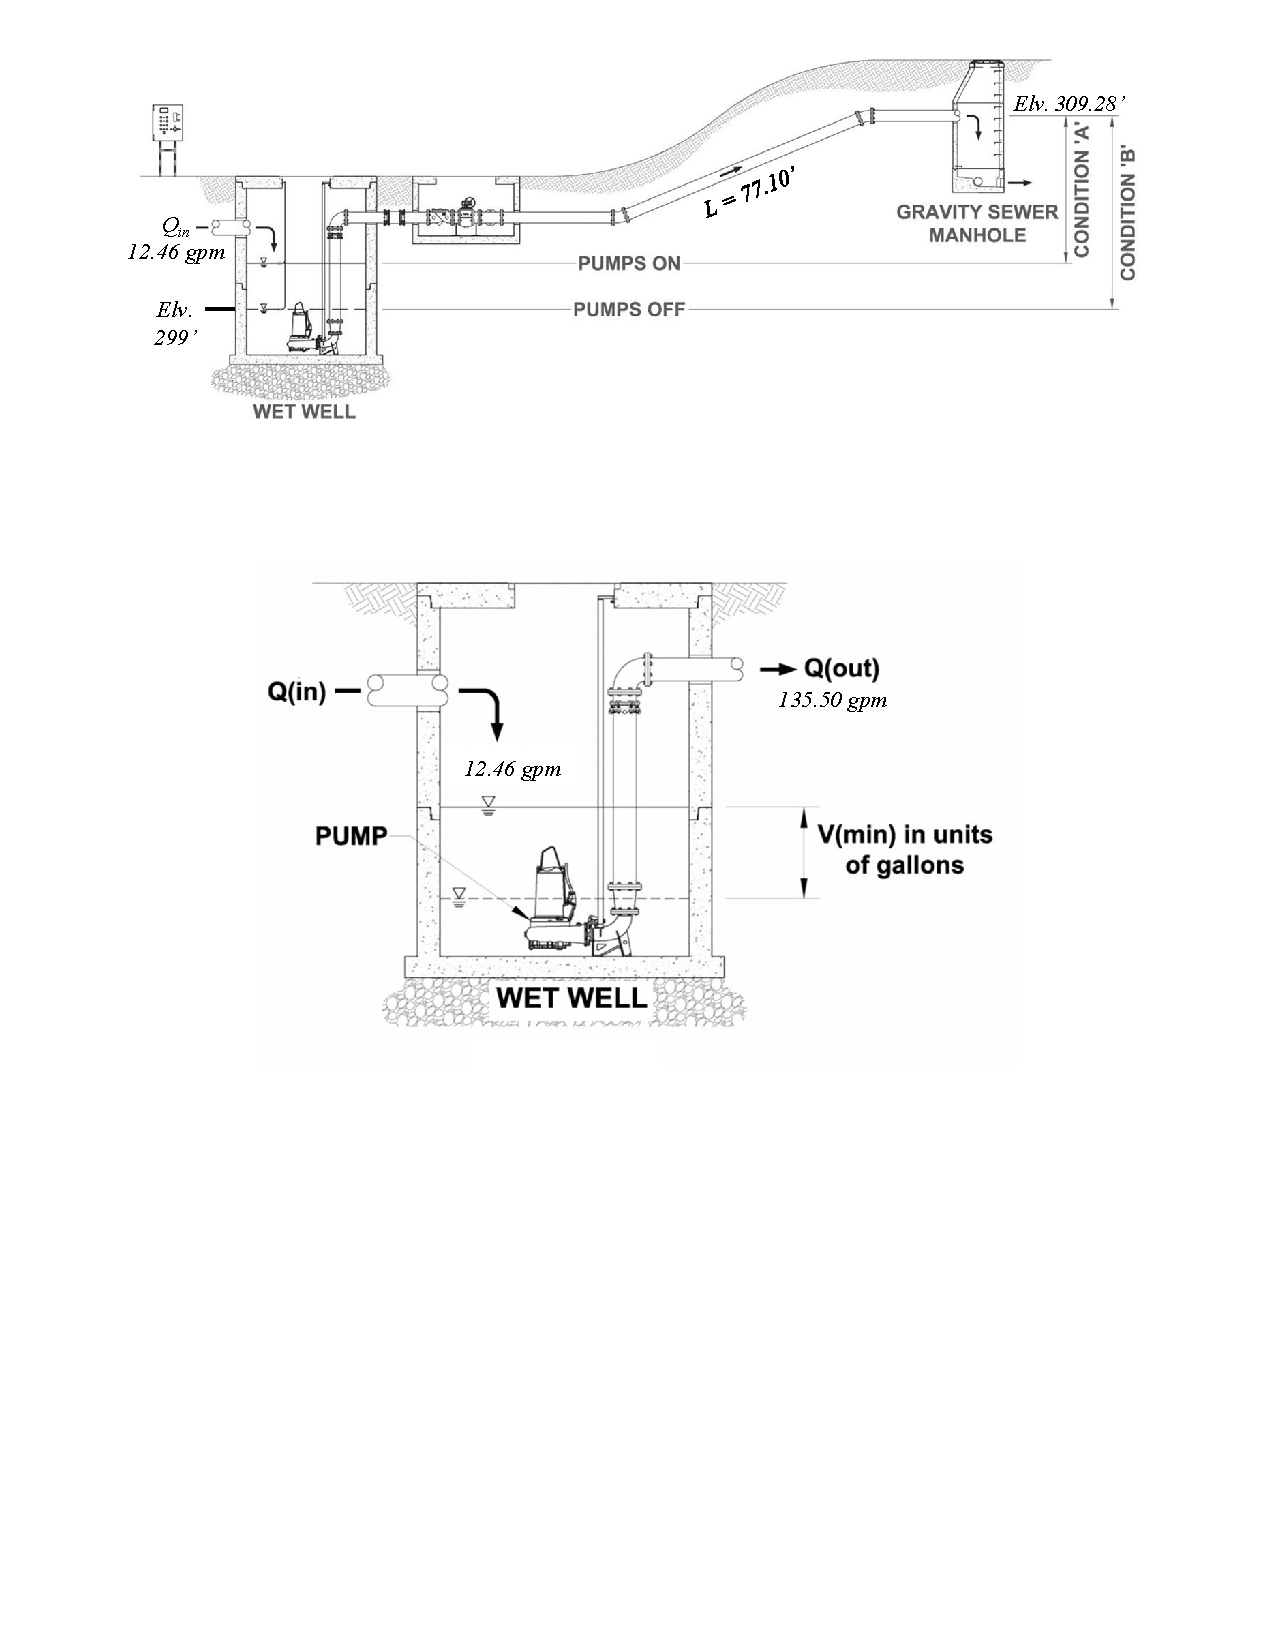
\includegraphics[
width=\textwidth,
trim={1.5in 4in 1.5in 4in},
clip
]{forcemain_pump_figures.pdf}
\caption{Wet well storage volume and inflow--outflow concept used for minimum storage calculations.}
\label{fig:wetwell_storage_volume}
\end{figure}

As shown in Figure~\ref{fig:wetwell_storage_volume}, the active storage region corresponds to the vertical distance between the pump-off and lead pump-on elevations within the wet well.

% -------------------------------------------------
\subsection{Hatch Sizing}
% -------------------------------------------------

After establishing the active storage requirement, the next step was to determine the minimum hatch opening needed for a duplex installation. The Sulzer installation dimension sheet for the XFP100C VX wet well installation shows that the recommended minimum opening for two pumps is $28~\text{in} \times 56~\text{in}$ on the U.S. dimension sheet, which was adopted directly for this design. The pump layout and minimum opening requirement are illustrated in Figure~\ref{fig:pump_install_dims}.

\begin{figure}[H]
\centering
\includegraphics[
width=0.9\textwidth,
page=2,
trim={0.2in 0.2in 0.2in 0.2in},
clip
]{dimension_ANM22624.pdf}
\caption{Installation dimensions for Sulzer XFP100C VX pump showing recommended hatch opening.}
\label{fig:pump_install_dims}
\end{figure}

As illustrated in Figure~\ref{fig:pump_install_dims}, the hatch opening must accommodate both pumps, their guide rail arrangement, lifting access, and the discharge hardware. The selected minimum hatch size for the wet well is therefore

\[
\boxed{28~\text{in} \times 56~\text{in}}
\]

This hatch dimension was not used by itself to select the wet well diameter. It was treated as the starting geometric requirement, and then the wet well diameter was checked against circular fit, pump clearances, and the discharge hardware inside the wet well.

Additional considerations for hatch design include loading classification, corrosion resistance, non-skid surfaces, and safety grates in accordance with industry practices \cite{Jensen_PumpStationDesignGuidelines_2012}.

% -------------------------------------------------
\subsection{Wet Well Diameter and Geometry}
% -------------------------------------------------

Most packaged lift stations utilize circular wet wells because round structures provide several advantages, including greater structural strength under soil pressure, lower construction cost, a smaller surface footprint, and simpler installation and precast manufacturing. A circular wet well was therefore selected for the Colebrooke station because round wet wells are standard for packaged duplex submersible lift stations and are structurally efficient for buried installation \cite{Jensen_PumpStationDesignGuidelines_2012}. Once the hatch size was known, the wet well diameter was evaluated. The first check was the geometric compatibility of the rectangular hatch with a circular wet well. The hatch diagonal is

\[
\begin{aligned}
d &= \sqrt{28^2+56^2} \\
&= \sqrt{784+3136} \\
&= \sqrt{3920} \\
&= 62.61~\text{in}
\end{aligned}
\]

Therefore, the wet well inside diameter must be greater than $62.61~\text{in}$ simply to accommodate the hatch geometry.

The next check was internal constructability. The selected pump is a DN100 unit with DN100 suction outlet and DN100 discharge outlet, which corresponds to a $4$-in connection. For a typical $4$-in flanged discharge connection, a reasonable working flange envelope of about $9~\text{in}$ outside diameter was assumed, with additional clearance required for the duckfoot elbow, guide rail connection, and contractor access for bolt tightening. The Sulzer installation sheet also shows a pump width of about $11.8~\text{in}$ in plan, and the discharge elbow and rail arrangement occupy additional horizontal space within the wet well. Because of this, selecting a wet well diameter only slightly larger than the hatch diagonal would leave insufficient room for the discharge elbow, flange, wall clearance, and maintenance access.

For that reason, the next standard practical diameter above the geometric minimum was adopted:

\[
\boxed{D_{well}=6~\text{ft ID}}
\]

This provides a $72$-in inside diameter, which exceeds the $62.61$-in hatch diagonal by

\[
\begin{aligned}
72-62.61 &= 9.39~\text{in}
\end{aligned}
\]

and also provides a workable margin for the $4$-in discharge hardware and wall clearances. This selection follows the same logic discussed in the Jensen guidance, namely that the hatch may geometrically fit but the well should be increased as needed to accommodate flanges, bends, and contractor working space \cite{Jensen_PumpStationDesignGuidelines_2012}. The selected $6$-ft-diameter well therefore represents a practical and constructible size rather than a purely geometric minimum.

% -------------------------------------------------
\subsection{Control Elevations}
% -------------------------------------------------

After determining the wet well size and minimum storage volume, the vertical control elevations that govern pump operation are established. In a duplex pumping system, five key control elevations are required:

\begin{enumerate}
\item Pump inlet elevation
\item Pump-off elevation
\item Lead pump-on elevation
\item Lag pump-on elevation
\item High water alarm elevation
\end{enumerate}

\begin{figure}[H]
\centering
\includegraphics[
width=\textwidth,
page=2,
trim={1.5in 2.5in 1in 4in},
clip
]{forcemain_pump_figures.pdf}
\caption{Wet well control elevations including pump-off, lead pump-on, lag pump-on, and high water alarm levels.}
\label{fig:wetwell_control_levels}
\end{figure}

As shown in Figure~\ref{fig:wetwell_control_levels}, the selected design values for the control increments are about $14~\text{in}$, $14.2~\text{in}$, $6~\text{in}$, and $12~\text{in}$ for $H_x$, $H_{min}$, $H_{lag}$, and $H_{res}$, respectively.

% -------------------------------------------------
\subsection{Minimum Submergence ($H_x$)}
% -------------------------------------------------

Once the wet well diameter and pump arrangement were fixed, the minimum submergence between the pump inlet and the pump-off water level was calculated to prevent vortex formation and air entrainment. Hydraulic Institute guidance provides empirical relationships for determining the required submergence based on pump inlet diameter and velocity \cite{ANSI_HI_98_1998,Hecker_1987_Conclusions}.

The minimum submergence relation from Hecker is

\[
\begin{aligned}
H_x &= D(1+2.3F_D)
\end{aligned}
\]

where

\[
\begin{aligned}
F_D &= \frac{V}{\sqrt{gD}}
\end{aligned}
\]

For the selected pump:

suction diameter $D=\text{DN100}=3.94~\text{in}=0.328~\text{ft}$
and pump discharge $Q=135.5~\text{gpm}$

Converting flow to cubic feet per second,

\[
\begin{aligned}
Q &= \frac{135.5}{448.83} \\
&= 0.302~\text{cfs}
\end{aligned}
\]

The suction area is

\[
\begin{aligned}
A &= \frac{\pi D^2}{4} \\
&= \frac{\pi(0.328)^2}{4} \\
&= 0.0845~\text{ft}^2
\end{aligned}
\]

The inlet velocity is

\[
\begin{aligned}
V &= \frac{Q}{A} \\
&= \frac{0.302}{0.0845} \\
&= 3.57~\text{ft/s}
\end{aligned}
\]

The hydraulic Froude number is

\[
\begin{aligned}
F_D &= \frac{3.57}{\sqrt{32.2(0.328)}} \\
&= \frac{3.57}{3.25} \\
&= 1.10
\end{aligned}
\]

Substituting into the submergence equation,

\[
\begin{aligned}
H_x &= 0.328(1+2.3\times 1.10) \\
&= 0.328(1+2.53) \\
&= 0.328(3.53) \\
&= 1.16~\text{ft}
\end{aligned}
\]

\[
\begin{aligned}
H_x &= 1.16\times 12 \\
&= 13.9~\text{in}
\end{aligned}
\]

Thus, the required minimum submergence is

\[
\boxed{H_x=14~\text{in}}
\]

The Sulzer installation dimension sheet indicates a water level dimension of $12.3~\text{in}$ for the selected installation arrangement. Because the calculated submergence requirement is larger, the design adopted the more conservative value of $14~\text{in}$.

% -------------------------------------------------
\subsection{Minimum Storage Depth ($H_{min}$)}
% -------------------------------------------------

The vertical distance between the pump-off elevation and the lead pump-on elevation is determined from the active wet well storage volume and wet well cross-sectional area. The governing design active storage was taken as $250~\text{gal}$. Converting this volume to cubic feet,

\[
\begin{aligned}
V &= 250\times 0.13368 \\
&= 33.42~\text{ft}^3
\end{aligned}
\]

For a $6$-ft-diameter circular wet well, the cross-sectional area is

\[
\begin{aligned}
A &= \pi r^2 \\
&= \pi(3)^2 \\
&= 28.27~\text{ft}^2
\end{aligned}
\]

Therefore,

\[
\begin{aligned}
H_{min} &= \frac{V}{A} \\
&= \frac{33.42}{28.27} \\
&= 1.18~\text{ft}
\end{aligned}
\]

\[
\begin{aligned}
H_{min} &= 1.18\times 12 \\
&= 14.2~\text{in}
\end{aligned}
\]

Thus, the required storage depth between pump-off and lead pump-on elevations is

\[
\boxed{H_{min}=14.2~\text{in}}
\]

% -------------------------------------------------
\subsection{Lag Pump Storage ($H_{lag}$)}
% -------------------------------------------------

For duplex stations with flows less than $200~\text{gpm}$, Jensen recommends a lag storage increment of at least $6~\text{in}$ \cite{Jensen_PumpStationDesignGuidelines_2012}. Since the selected pump discharge is $135.5~\text{gpm}$, the Colebrooke station falls within that range. Accordingly,

\[
\boxed{H_{lag}=6~\text{in}=0.5~\text{ft}}
\]

This is the vertical distance between the lead pump-on elevation and the lag pump-on elevation.

% -------------------------------------------------
\subsection{Reservoir Storage ($H_{res}$)}
% -------------------------------------------------

The reservoir storage between the lag pump-on elevation and the high water alarm is a factor of safety that provides emergency storage in the event of excessive inflow or pump malfunction. For small stations below $200~\text{gpm}$, Jensen recommends a minimum value of $12~\text{in}$ \cite{Jensen_PumpStationDesignGuidelines_2012}. Therefore,

\[
\boxed{H_{res}=12~\text{in}=1.0~\text{ft}}
\]

% -------------------------------------------------
\subsection{Summary of Wet Well Design Parameters}
% -------------------------------------------------

Based on the hydraulic calculations and equipment data, the recommended wet well configuration for the Colebrooke Subdivision pump station is summarized in Table~\ref{tab:wetwell_summary}.

\begin{table}[H]
\centering
\caption{Summary of recommended wet well design parameters}
\label{tab:wetwell_summary}
\begin{tabular}{ll}
\toprule
\textbf{Parameter} & \textbf{Value} \\
\midrule
Pump type & Sulzer XFP100C VX 1$\sim$ (wet pit) \\
Pump capacity & $135.5~\text{gpm}$ at $12.08~\text{ft}$ head \\
Impeller type & Vortex impeller \\
Wet well diameter & $6~\text{ft}$ inside diameter \\
Active storage volume & $250~\text{gal}$ \\
Minimum storage depth ($H_{min}$) & $14.2~\text{in}$ \\
Minimum submergence ($H_x$) & $14~\text{in}$ \\
Lag pump storage ($H_{lag}$) & $6~\text{in}$ \\
Reservoir storage ($H_{res}$) & $12~\text{in}$ \\
Recommended hatch opening & $28~\text{in} \times 56~\text{in}$ \\
\bottomrule
\end{tabular}
\end{table}

The selected control-elevation increments are

\[
H_x = 14~\text{in}, \qquad
H_{min} = 14.2~\text{in}, \qquad
H_{lag} = 6~\text{in}, \qquad
H_{res} = 12~\text{in}
\]

These design parameters ensure that the wet well provides sufficient hydraulic storage, safe pump operation, and reliable performance under both normal and peak flow conditions. The final configuration also satisfies regulatory design recommendations and operational guidelines for municipal wastewater lift stations \cite{MDEQ_DesignGuidance_2025,TenStates_RecommendedStandards_2014}.
